Algorytm wstecznej propagacji jest wykorzystywany do nauczania wielowarstwowych sieci jednokierunkowych.
Taka sieć zawiera warstwę wejściową i warstwę wyjściową,
może posiadać również warstwy ukryte (wykorzystywana do problemów liniowo nieseparowalnych).
Każda warstwa zawiera dowolną ilość neuronów.
Neurony są połączone ze sobą w taki sposób, że każdy neuron warstwy innej niż wyjściowa jest połączony z każdym neuronem kolejnej warstwy,
a każde połączenie ma określoną wagę.
Dodatkowo możliwe jest połączenie do tego zwanego biasa, czyli połączenia do neuronu, który zawsze przyjmuje wartość 1.
Połączenia wejściowe do neuronu będą wpływać na to jaką będzie miał wartość.

Kluczowym pytaniem jest to jak powinna wyglądać sieć obsługująca funkcję NXoR. 
Jako, że funkcja NXoR przyjmuje dwie liczby wejściu jasne jest, że powinna posiadać również dwa neurony wejściowe.
Wiemy również, że sieć posiada jedno wyjście, co sprawia, że potrzebujemy tylko jednego neuronu wyjściowego.

\begin{center}
  \begin{tabular}{||c c c||} 
  \hline
  x1 & x2 & NXoR \\ [0.5ex] 
  \hline\hline
  0 & 0 & 1\\ 
  \hline
  0 & 1 & 0 \\
  \hline
  1 & 0 & 0 \\
  \hline
  1 & 1 & 1 \\ [0.5ex] 
  \hline
 \end{tabular}
 \end{center}
 
W powyższym opisie pojawiła się wzmianka o tym, że warstwa ukryta jest wykorzystywana w problemach, które nie są liniowo separowalne.
W związku z tym należy się zastanowić czy problem NXoR do takowych należy.
Aby sprawdzić czy problem jest liniowo separowalny należy narysować na płaszczyźnie punkty w których funkcja przyjmuje 0 i tych w których przyjmuje 1, a następnie sprawdzić czy istnieje prosta, która przedzieli te punkty na dwie płaszczyzny.
Jak pokazuje rysunek \ref{fig:separability} do funkcji spełniających ten warunek należą funkcje AND i OR.
Natomiast przykładem funkcji niespełniającej tego warunku jest XOR, a więc też jego odwrotność czyli NXoR.
W związku z tym będziemy potrzebować warstwy ukrytej.
 
\begin{figure}[!ht]
  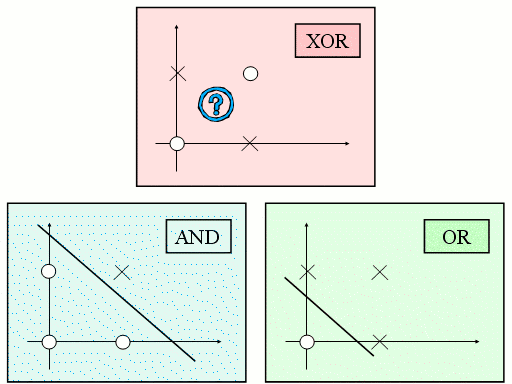
\includegraphics[width=\linewidth]{images/andorxor.png}
  \source{https://edux.pjwstk.edu.pl/mat/2144/lec/rW2.htm/}
  \caption{Liniowa separowalność funkcji AND, OR, XOR}
  \label{fig:separability}
\end{figure}

Otwartym pytaniem pozostaje natomiast to ile neuronów powinna posiadać ta warstwa.
Tutaj posłużymy się cytatem z książki Jeffa Heatona "Introduction to Neural Networks for C\#":
\begin{quote}
  There are many rule-of-thumb methods for determining the correct number of neurons to use in the hidden layers, such as the following:
  \begin{itemize}
    \item  The number of hidden neurons should be between the size of the input layer and the size of the output layer.  
    \item   The number of hidden neurons should be 2/3 the size of the input layer, plus the size of the output layer.
    \item   The number of hidden neurons should be less than twice the size of the input layer.
  \end{itemize}
\end{quote}

W związku z powyższym nasza warstwa ukryta będzie zawierała 2 neurony.

Kolejnym pytaniem jest to czy należy wprowadzać biasa.
Wstępne testy pokazały, że jego obecność przyśpiesza trening sieci,
ale aby nie komplikować opisu zostanie on pominięty.

Ostatecznie nasza sieć będzie wyglądała tak jak na rysunku \ref{fig:architecture}

\begin{figure}[!ht]
  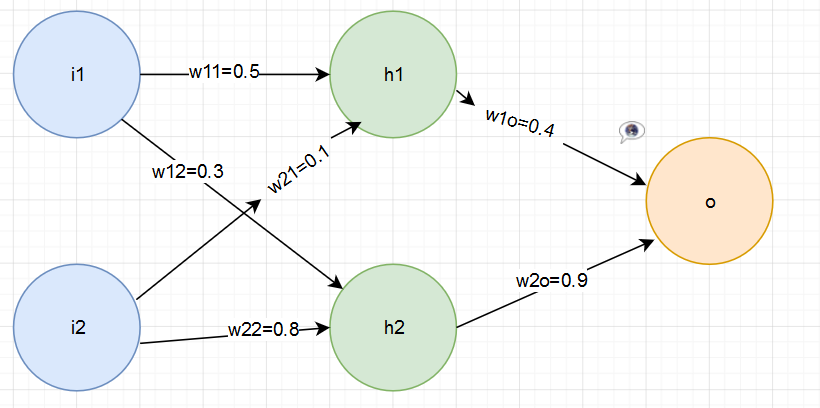
\includegraphics[width=\linewidth]{images/architecture.png}
  \caption{Architektura sieci realizującej funkcję NXoR}
  \label{fig:architecture}
\end{figure}

